\documentclass[a4paper]{article}

% Set for specific document
\def\DOCTITLE{CSC3621 Coursework 1 Exercise 3}
\def\DOCAUTHOR{Dan Nixon (120263697)}
\def\DOCDATE{16/10/2015}

% Set document attributes
\title{\DOCTITLE}
\author{\DOCAUTHOR}
\date{\DOCDATE}

\usepackage{fullpage}
\usepackage{scrextend}
\usepackage{titlesec}
\usepackage{fancyhdr}
\usepackage[section]{placeins}
\usepackage{minted}

% Handle graphics correctly
\ifx\pdftexversion\undefined
\usepackage{graphicx}
% \usepackage[dvips]{graphicx}
\else
\usepackage[pdftex]{graphicx}
\DeclareGraphicsRule{*}{mps}{*}{}
\fi

% Setup headers and footers
\pagestyle{fancy}
\lhead{}
\chead{\DOCTITLE}
\rhead{}
\rfoot{\DOCDATE}
\cfoot{\thepage}
\lfoot{\DOCAUTHOR}

% Set header and footer sizes
\renewcommand{\headrulewidth}{0.4pt}
\renewcommand{\footrulewidth}{0.4pt}
\setlength{\headheight}{15.2pt}
\setlength{\headsep}{15.2pt}

\begin{document}

\section{One time pad encryption program}

The one time pad program is split between pad generation
(\texttt{OneTimePadGenerator.java}) and encryption/decryption
(\texttt{OneTimePadEncryption.java}). The program is used through a command line
interface implemented in \texttt{OneTimePadApp.java} with the following
arguments:

\begin{description}
  \item[\texttt{--generate-pad-file FILE}]
    Generate a pad and save it as \texttt{FILE}.
  \item[\texttt{--length N}]
    Set the length of the generated pad to be \texttt{N} bytes.
  \item[\texttt{--seed N}]
    Sets the seed of the pad generator to \texttt{N} otherwise the seed is set
    by equation \ref{eq:clock_seed}.
  \item[\texttt{--encrypt}]
    Encrypt a message file.
  \item[\texttt{--decrypt}]
    Decrypt an encrypted message.
  \item[\texttt{--pad-file FILE}]
    The pad file to use during encryption or decryption.
  \item[\texttt{--message-file FILE}]
    The message file to be encrypted.
  \item[\texttt{--cipher-file FILE}]
    The file to read/save the cipher to/from.
\end{description}

\subsection{Pad file generation}

Generation of the one time pad is done by generating a random array of bytes
using the \\ \texttt{java.security.SecureRandom} random number generator using a
byte array of length 8 (determined by the value of a long integer) as the seed.

This generator is implemented as the \texttt{generateOneTimePad(int, int)}
method in the \texttt{OneTimePadGenerator} class. There is also a
\texttt{generateOneTimePad(int)} method that only takes the length of the pad as
a parameter, in this case the system clock is used for the seed.

Figure \ref{fig:generate_pad} shows the result of generating a 1MB one time pad
using a set integer key and the first 240 bytes of the hex dump of the generated
pad file.

\begin{figure}[h!]
  \centering
  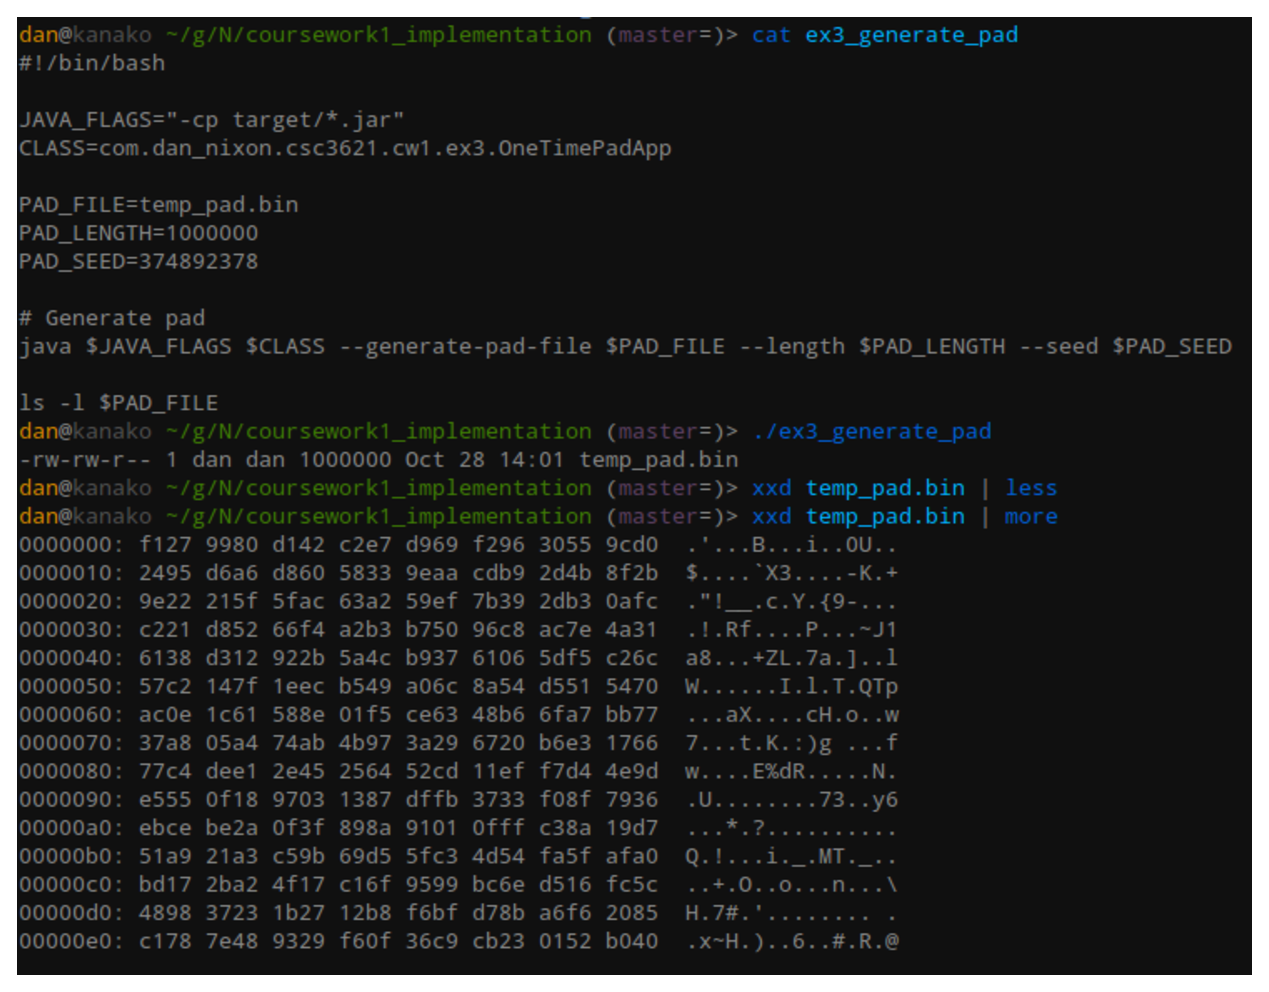
\includegraphics[width=0.55\textwidth]{graphics/ex3_pad_generation.eps}
  \caption{Generation of a one time pad}
  \label{fig:generate_pad}
\end{figure}

\subsection{Encryption and decryption}

Once the pad has been generated encryption and decryption are simple XOR
operations over the pad and message/cipher text arrays (equations
\ref{eq:encrypt} and \ref{eq:decrypt} respectively).

\begin{equation}
  C_{i} = P_{i} \oplus M_{i}
  \label{eq:encrypt}
\end{equation}
\FloatBarrier

\begin{equation}
  M_{i} = P_{i} \oplus C_{i}
  \label{eq:decrypt}
\end{equation}
\FloatBarrier

where $M$ is the plain text message, $P$ is the one time pad and $C$ is the
cipher text.

This functionality is implemented in the \texttt{OneTimePadEncryption} Java
class, specifically the \texttt{encrypt()} and \texttt{decrypt()} methods.

\subsection{Correctness}

The correctness of the encryption and decryption operations is tested using a
unit test in the \\ \texttt{OneTimePadEncryoptionTest.java} file, amongst other
tests this tests the encryption and decryption of the test vector given in the
specification to validate the two operations.

In addition to this I also performed a encryption and decryption cycle on the
plain text from exercise 1 to ensure that a sample of plain text survives the
encryption/decryption cycle intact.

This can be executed using the \texttt{ex3\_encrypt\_decrypt\_cycle} Bash
script. The result of this are shown in figure \ref{fig:enc_dec_cycle}.

\begin{figure}[h!]
  \centering
  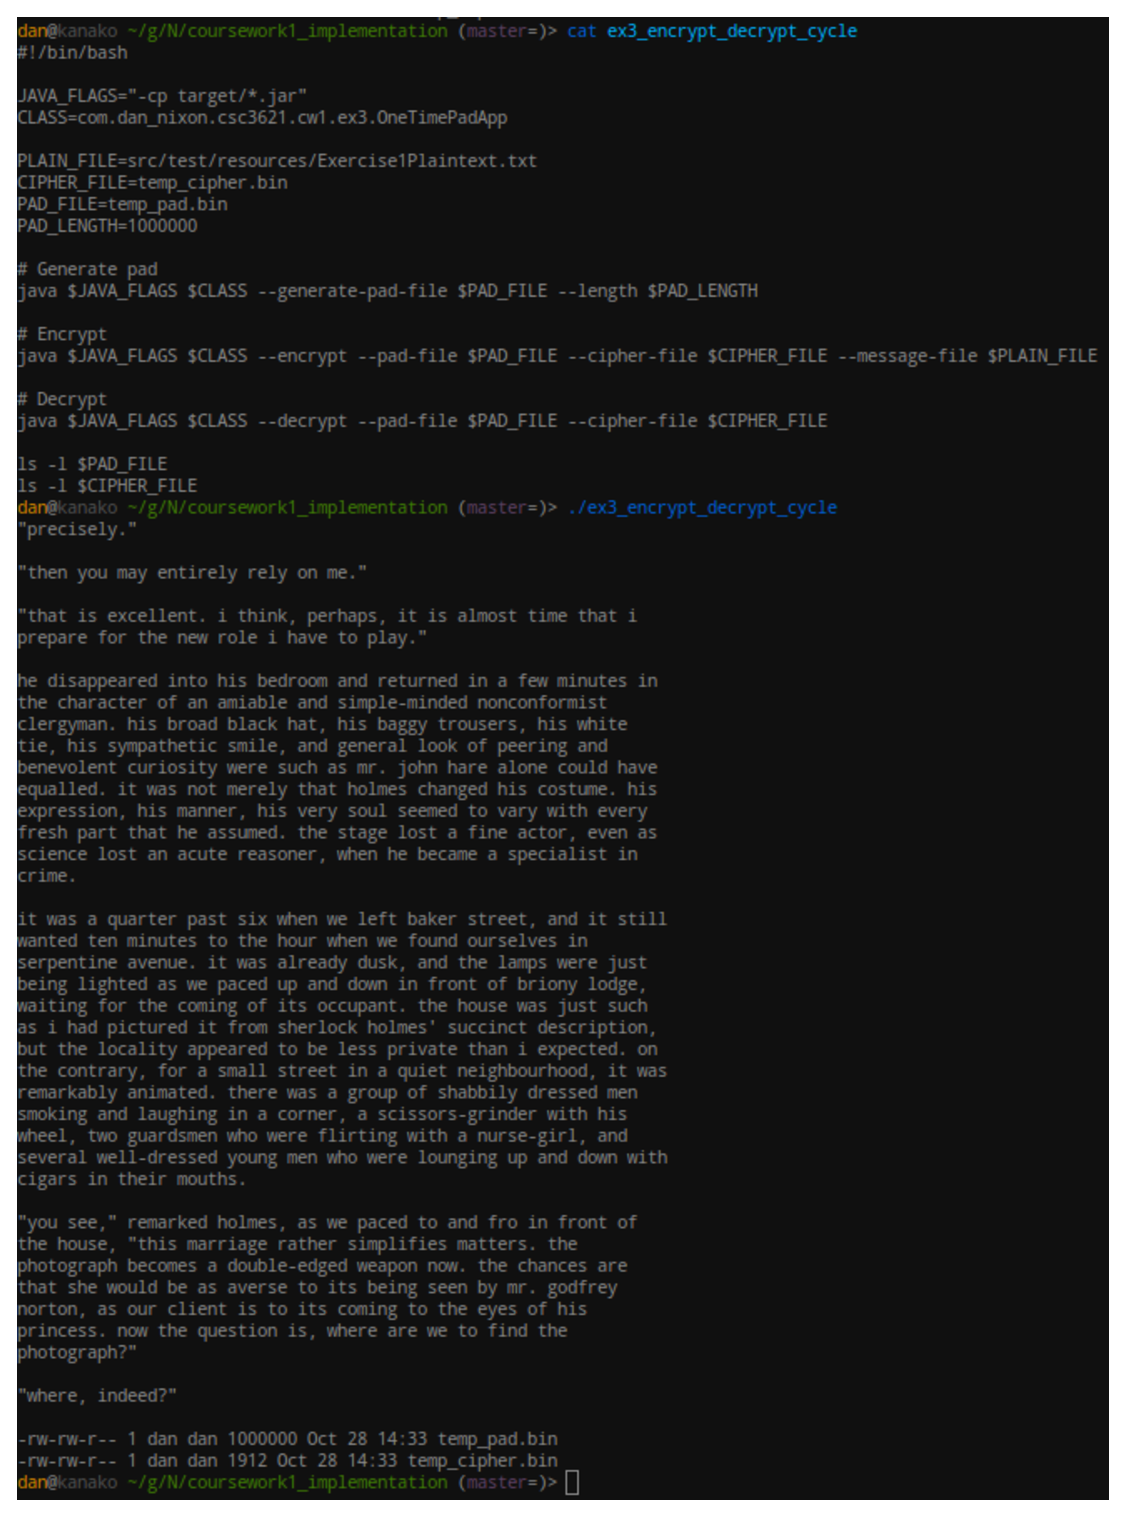
\includegraphics[width=0.55\textwidth]{graphics/ex3_enc_dec_cycle.eps}
  \caption{Encryption and decryption cycle}
  \label{fig:enc_dec_cycle}
\end{figure}

When the program was tested using a pad and cipher generated by the program
written by another student it was able to correctly decrypt the message, the
same was true for their program being able to decrypt messages generated with my
program.

\section{Cryptanalysis of cipher data}

The key to the successful cryptanalysis of the two time pad attack is that when
a space (\texttt{0x20}) is XORed with a uppercase or lowercase alphabetic
character then the case of that character is negated.

For instance $0x64 \  \mathrm{(d)} \oplus 0x20 = 0x44 \  \mathrm{(D)}$.

This means that when the XOR of two cipher texts is taken any bytes that can be
converted to ASCII alphabetical characters the string produced (in the
implementation and this document known as the "analysis string") indicate that
the character in the same position in one of the messages was a space whilst the
other was the same letter in the opposite case.

For instance, one can determine given the XOR string
\texttt{--UN-} that the third character of one message was a space whilst the
third character of the other message was lowercase \textit{u}.

When multiple cipher texts are available this technique can be used to analyse
multiple XOR strings at once, where the target cipher text is XORed with
multiple other cipher texts.

When these strings are analysed per column you can then determine what character
belongs in the same position of the target cipher text. Considering all bytes in
a column that have ASCII alphabetical representations, if all are the same
character then that is the character in the same column of the target message,
otherwise if there are a mixture of characters then this indicates a space in
the target message.

For instance, figure \ref{fig:cryptanalysis_eg} shows the analysis strings for
the target cipher text in this exercise, from this you can determine that the
third character in the message must be \textit{u}, given that it is the unique
character in the third column. Likewise the fourth character of the message must
be a space as the fourth column contains multiple different characters.

\begin{listing}
  \inputminted[frame=lines,fontsize=\scriptsize,firstline=52,lastline=57]{text}{listings/ex3_cryptanalysis_1.txt}
  \caption{Cryptanalysis example}
  \label{listing:cryptanalysis_eg}
\end{listing}
\FloatBarrier

With this knowledge it is simple to write a program that will perform this
analysis automatically and generate a string that best matches the plain text
message for a given cipher text. This was implemented in the \texttt{OTPAttack}
Java class (part of which is based on the \texttt{OTPAttack.java} program
supplied with the specification).

Figure \ref{fig:cryptanalysis} shows the output of this program when executed
using the \texttt{ex3\_cryptanalysis} Bash script, listing
\ref{listing:cryptanalysis_verbose} shows the full verbose output including the
analysis strings for each of the cipher texts included in the specification.

\begin{figure}[h!]
  \centering
  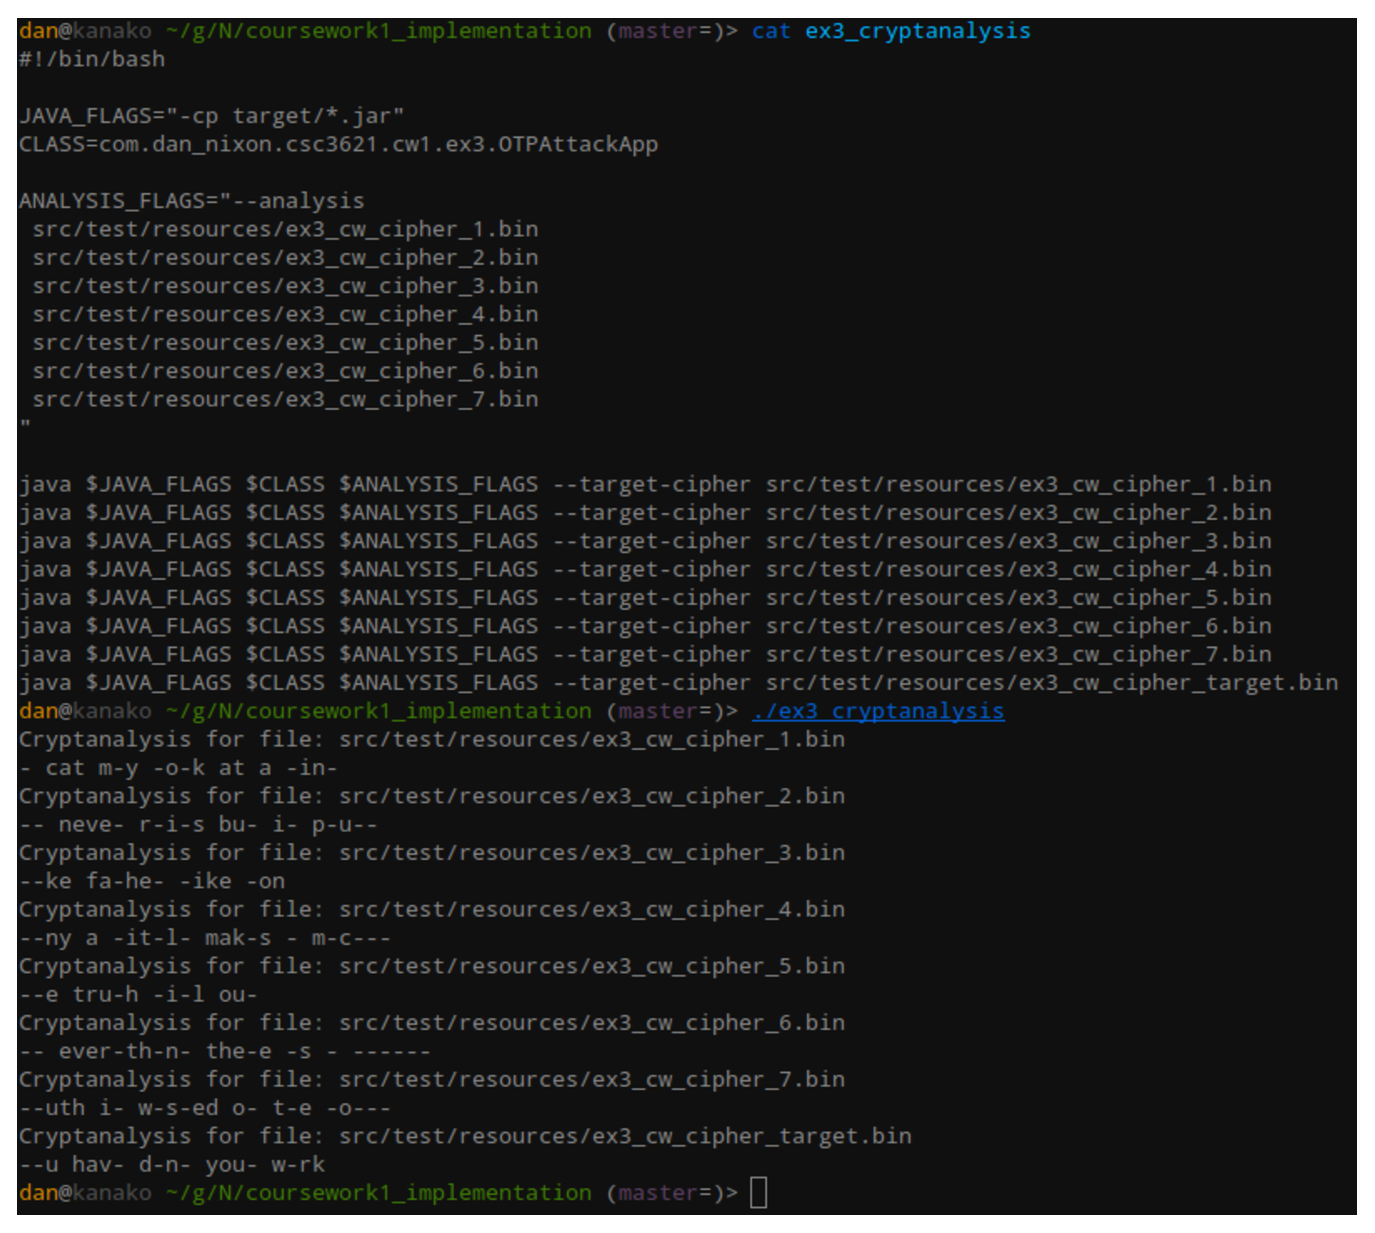
\includegraphics[width=0.55\textwidth]{graphics/ex3_cryptanalysis_1.eps}
  \caption{Execution of cryptanalysis program}
  \label{fig:cryptanalysis}
\end{figure}

\begin{listing}
  \inputminted[frame=lines,fontsize=\scriptsize]{text}{listings/ex3_cryptanalysis_1.txt}
  \caption{Verbose output of cryptanalysis program}
  \label{listing:cryptanalysis_verbose}
\end{listing}

This program obtains reasonable guesses for the plain text messages for each of
the cipher texts, at this point the full contents of all messages is easy to
obtain by intuition; the seven sample cipher texts all seem to be famous quotes
and the target cipher text contains enough known characters to be identified
easily. The guessed messages and deciphered messaged are given in table
\ref{tab:deciphered_messages}.

\begin{table}[h]
  \centering
  \begin{tabular}{lll}
    \hline
    Ciphertext  & Analysis                                  & Message                         \\
    \hline
    1           & \texttt{- cat m-y -o-k at a -in-}         & A cat may look at a king        \\
    2           & \texttt{-- neve- r-i-s bu- i- p-u--}      & It never rains but it pours     \\
    3           & \texttt{--ke fa-he- -ike -on}             & Like father like son            \\
    4           & \texttt{--ny a -it-l- mak-s - m-c---}     & Many a little makes a mickle    \\
    5           & \texttt{--e tru-h -i-l ou-}               & The truth will out              \\
    6           & \texttt{-- ever-th-n- the-e -s - ------}  & In everything there is a season \\
    7           & \texttt{--uth i- w-s-ed o- t-e -o---}     & Youth is wasted on the young    \\
    Target      & \texttt{--u hav- d-n- you- w-rk}          & You have done your work         \\
    \hline
  \end{tabular}
  \caption{Deciphered messages}
  \label{tab:deciphered_messages}
\end{table}

\subsection{Obtaining the original key}

I also made an effort to retrieve the original pad used to encrypt the target
cipher text, this is done using a program to do a simple XOR across two byte
arrays and is executed using the \texttt{ex3\_retrieve\_pad} Bash script.

The output of this program is shown in figure \ref{fig:retrieve_pad}

\begin{figure}[h!]
  \centering
  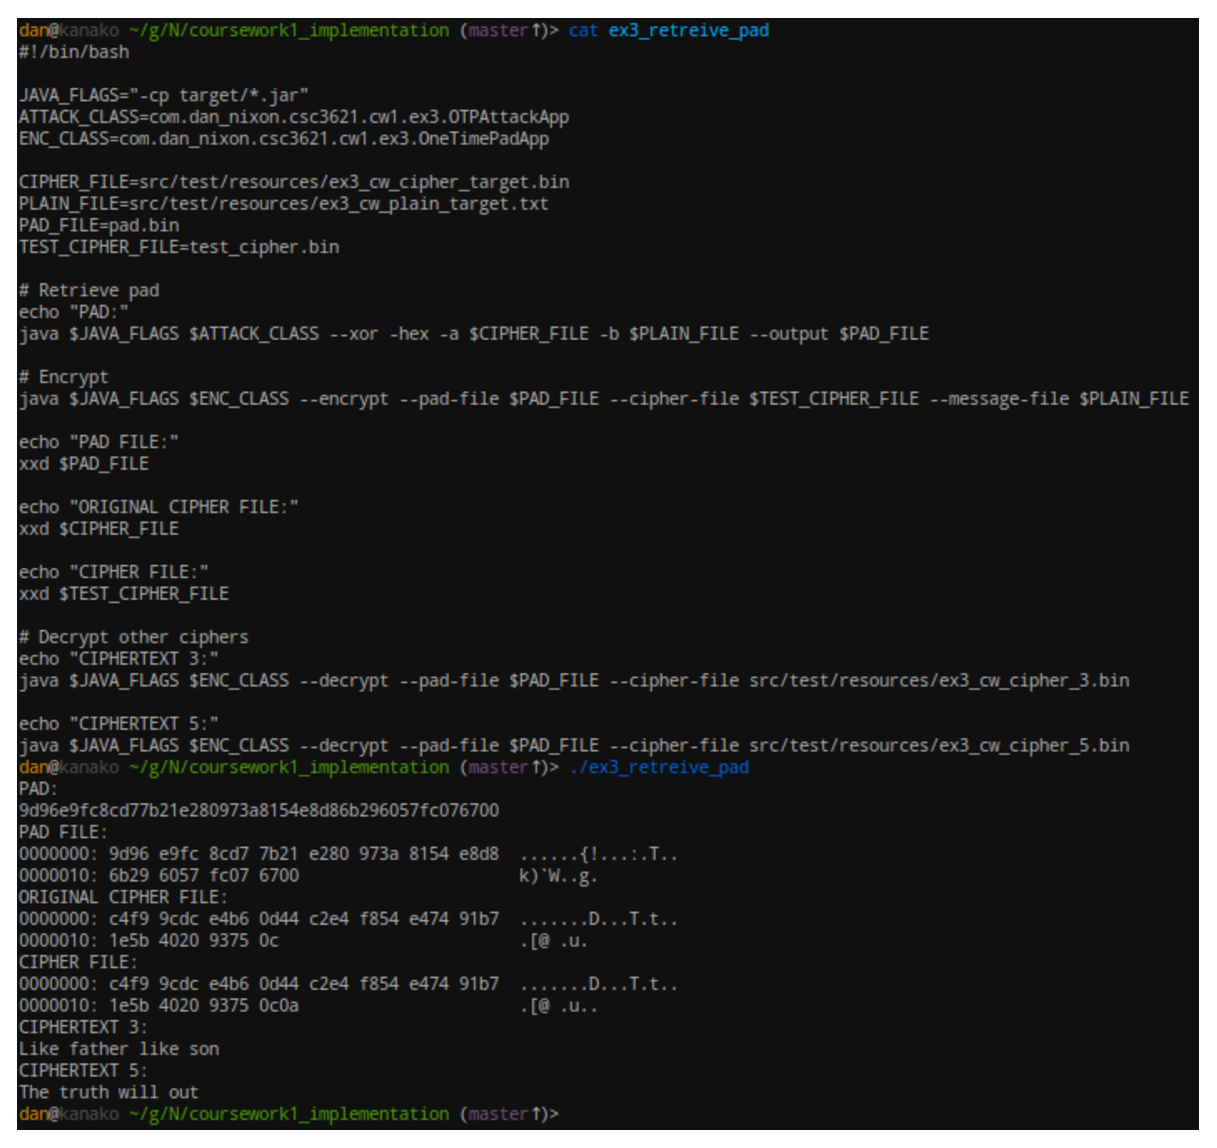
\includegraphics[width=0.55\textwidth]{graphics/ex3_obtain_pad.eps}
  \caption{Retrieval of original pad}
  \label{fig:retrieve_pad}
\end{figure}

This shows that the pad used to encrypt the target cipher text was \\
\texttt{9d96e9fc8cd77b21e280973a8154e8d86b296057fc0767}, assuming that the
message started with a capital letter (note that the pad shown in the figure has
an additional \texttt{0x00} at the end of the pad, this is caused by the newline
character when the plain text is loaded from a file).

\end{document}
